%%%%%%%%%%%%%%%%%%%%%%%%%%%%%%%%%%%%%%%%%%%%%%%%%%%%%%%%%%%%%%%%%%%%%%%%%%%%%%%%
%2345678901234567890123456789012345678901234567890123456789012345678901234567890
%        1         2         3         4         5         6         7         8

\documentclass[letterpaper, 10 pt, conference]{ieeeconf}  % Comment this line out
                                                          % if you need a4paper
%\documentclass[a4paper, 10pt, conference]{ieeeconf}      % Use this line for a4
                                                          % paper

\IEEEoverridecommandlockouts                              % This command is only
                                                          % needed if you want to
                                                          % use the \thanks command
\overrideIEEEmargins

% The following packages can be found on http:\\www.ctan.org
\usepackage{graphics} % for pdf, bitmapped graphics files
\usepackage{epsfig} % for postscript graphics files
\usepackage{mathptmx} % assumes new font selection scheme installed
\usepackage{times} % assumes new font selection scheme installed
\usepackage{amsmath} % assumes amsmath package installed
\usepackage{amssymb}  % assumes amsmath package installed
\usepackage{minted}
\usepackage{lipsum, babel}
\usepackage[options ]{algorithm2e}
\usepackage{graphics}
\usepackage{graphicx}
\usepackage[colorlinks = true,
            linkcolor = blue,
            urlcolor  = blue,
            citecolor = blue,
            anchorcolor = blue]{hyperref}
\usepackage[toc,page]{appendix}
\graphicspath{ {images/} }

\title{\LARGE \bf
Resource constrained scheduling with Dual-port memory
}


\author{Shreshth Tuli% <-this % stops a space
}


\begin{document}



\maketitle
\thispagestyle{empty}
\pagestyle{empty}


%%%%%%%%%%%%%%%%%%%%%%%%%%%%%%%%%%%%%%%%%%%%%%%%%%%%%%%%%%%%%%%%%%%%%%%%%%%%%%%%
\begin{abstract}

This report explains the details of implementing a resource constrained scheduling algorithm using C++. Details about the model, design decisions and testing have been elaborated to justify the correctness of the work.

\end{abstract}


%%%%%%%%%%%%%%%%%%%%%%%%%%%%%%%%%%%%%%%%%%%%%%%%%%%%%%%%%%%%%%%%%%%%%%%%%%%%%%%%
\section{INTRODUCTION}

The scheduling problem in high-level synthesis is concerned with sequencing the operators of a control/data flow graph (CDFG) in correct order. This optimization problem, is specified in two ways: (1) resource constrained scheduling (RCS) minimizes the number of control steps when the number of FU's are fixed; (2) time-constrained scheduling (TCS) minimizes the number of resources when the number of control
steps is fixed. This work aims at solving the former problem using simple heuristics based approach and provide a near optimal schedule (considering the problem is NP-hard). \\
We assume the input to our solution is a Data Flow Graph (DFG) which may be specified as a labeled Graph. Using computation and transformations on this graph, we propose to reach the desired results.

\section{MODEL}

A fundamental step in building a solution would require a conceptual level modeling of the problem. A straightforward method for modeling a combinations circuit with the level of abstraction of that of a DFG, is using Graph data structure. We use a Directed Acyclic Graph (DAG) to represent the DFG, which can also be interpreted as a sequence diagram. 

\section{DESIGN DECISIONS}

For implementing the model specified, C++ Boost library was used. Boost library provided an elegant interface and appropriate data-structures to store the graph. To specify the cycle and resource number for each labelled node of the graph, we specify input in a labelled fashion. Now, in a sequence diagram it is necessary to specify labels for nodes but redundant for edges so that the program can output the cycle and resource numbers corresponding to the label specified in the input. Thus we use input label as an identifier for output specification. \\
Also, we include component delays and resource limits in the input specification. These two integers are assumed to be specified for a class of resources like Adder, Subtractor, Multiplier, memory Read and Memory Write, and not for each type of adder, etc. 

\section{ALGORITHM}

The algorithm used for the resource constrained scheduling is a heuristic based List scheduling algorithm. Using unconstrained scheduling algorithms like ASAP and ALAP, we obtain the earliest and the latest schedules for each node. Using these schedules, we calculate the Mobility heuristic of each node. This heuristic helps us to decide what order to schedule nodes when we have multiple options from the ready-list. For the purpose of this model of problem, we keep ready-list for each operation type. We list-schedule each of these operations independently as per the DFG sequence and dependence across nodes. To deal with multiple connected components of the input DFG, we connect these components with a dummy node in the end which is not displayed in the output, but is used to connect all these independent DAGs. A pseudocode of the approach is listed in \ref{alg:algo}. \\

\begin{algorithm}[H]
\label{alg:algo}
\SetAlgoLined
\KwResult{Schedule}
\textbf{Input:} Data flow graph \textit{G}, quantities \textit{q}, delays \textit{d}\\
 cycle = 1\;
 ready-list = \{\}\;
 \While{all nodes not scheduled}{
 \textit{ s} = ASAP schedule of \textit{G}\;
  \textit{s'} = ALAP schedule of \textit{G}\;
  \For{all nodes \textit{n} in \textit{G}}{
    \textit{mobility(n)} = \|\textit{s'(n)} - \textit{s(n)}\|\;
    
  }
  \textit{l} = {} = ready-list for each operation type\;
  \For{all nodes \textit{n} not scheduled in \textit{G}}{
    \eIf{inDegree of \textit{n} == 0}{
        append \textit{n} to \textit{l}
    }
  }
  sort (\textit{l}, with increasing mobility value)\;
  \For{resource type \textit{t} and integer \textit{i} in range 0 to \textbf{min}(\textit{q(t)}, size of \textit{l})}{
    node \textit{n} = \textit{l(i)}\;
    \eIf{inDegree of n in original graph == 0}{
        schedule of \textit{n} = 1\;
    }
    {
        schedule of \textit{n} = \textbf{max}(schedule of parent + delay of parent) over all parents of n\;
    }
  }
  remove scheduled nodes from \textit{G}\;
 }
 \caption{List Scheduling using Mobility}
\end{algorithm}

\begin{figure}[!h]
  \centering
  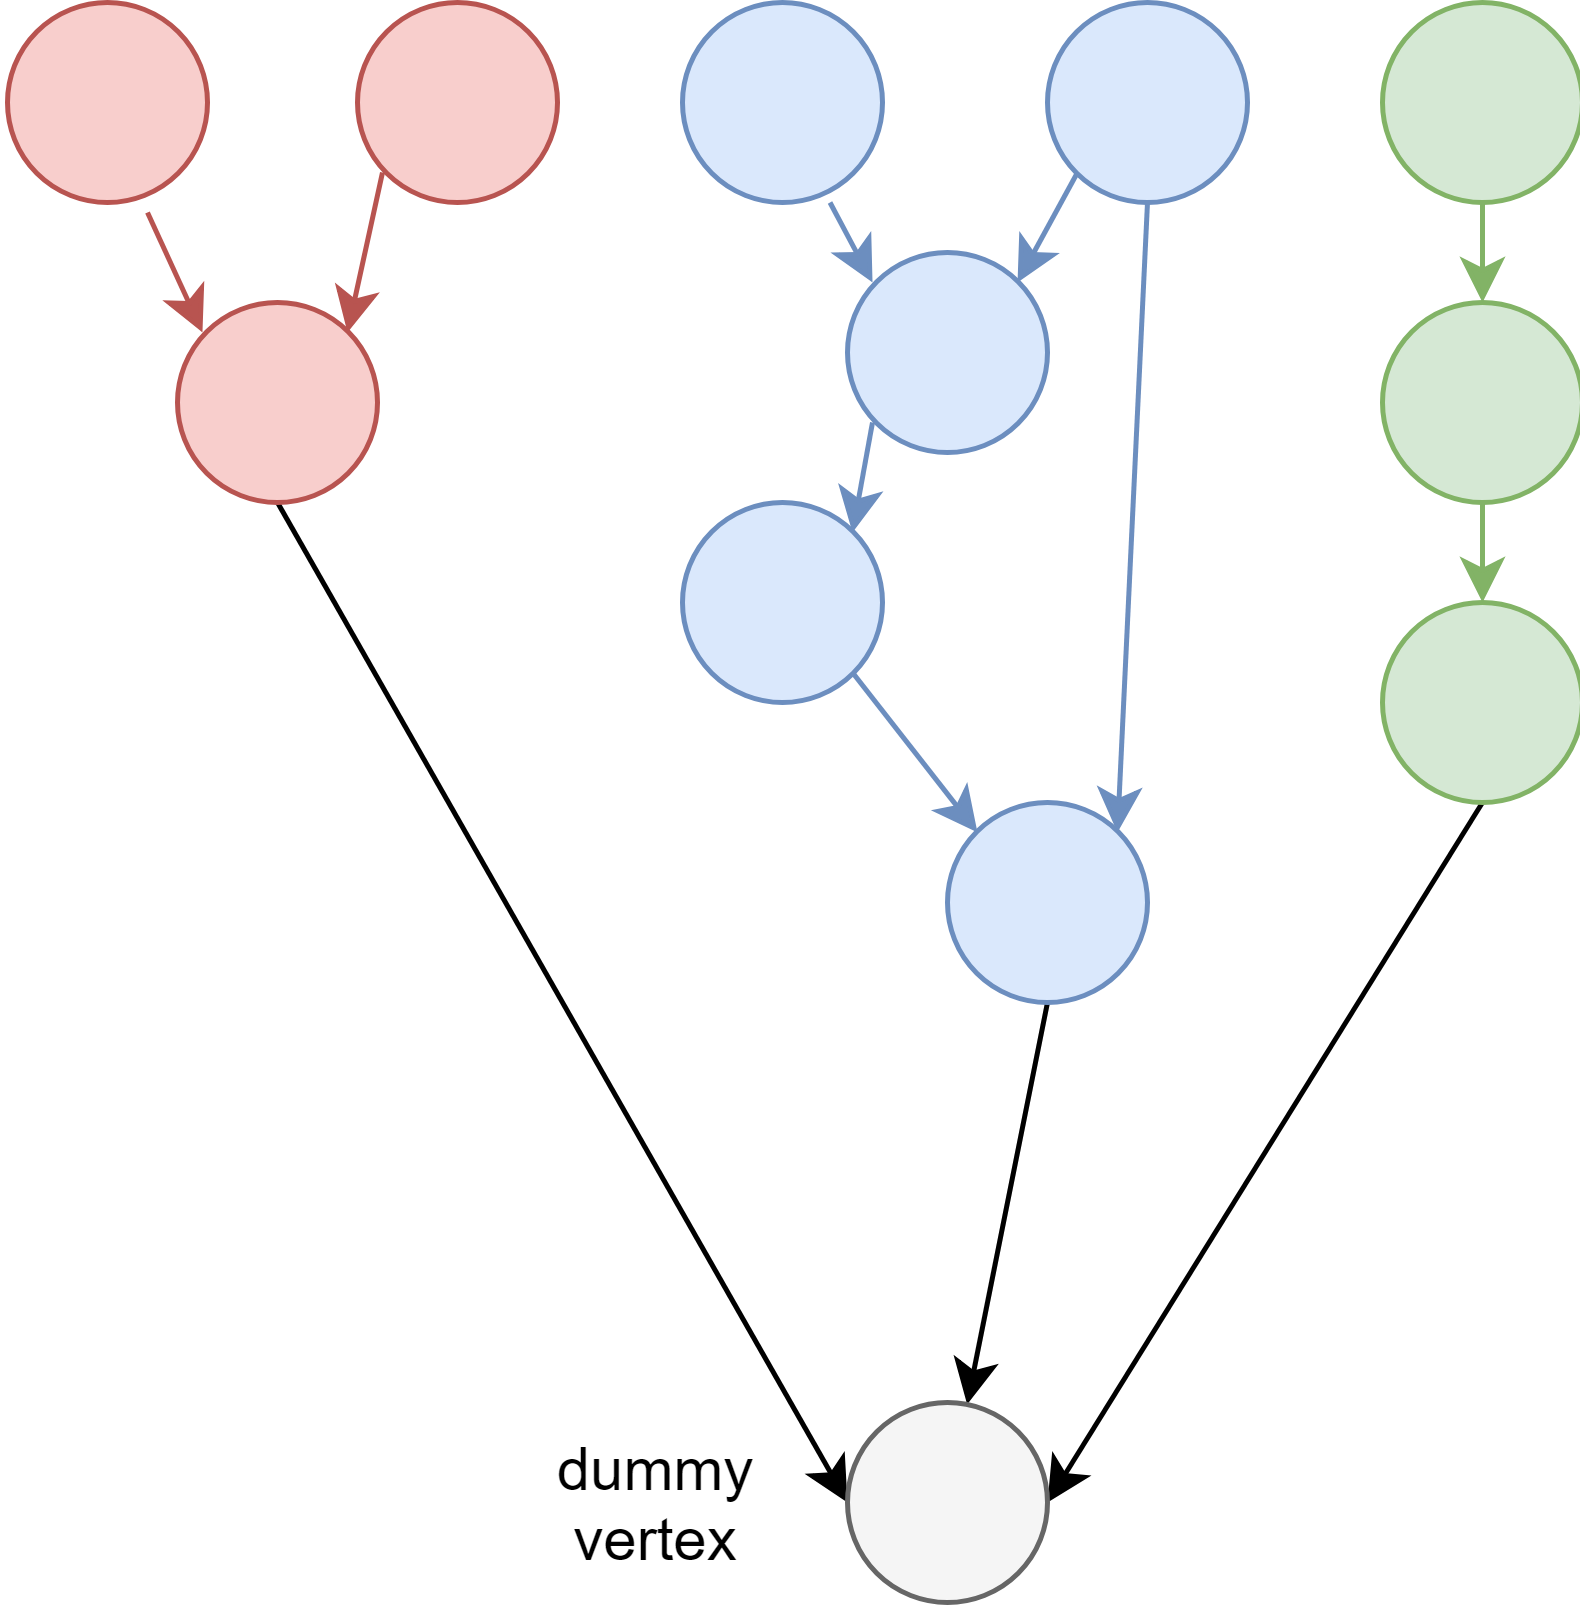
\includegraphics[width=65mm]{connect.png}
  \caption{Connecting disconnected components of DFG}
  \label{fig:connect}
\end{figure}

\section{IMPLEMENTATION}

\subsection{Graph representation}

The graph format used for the program was the Labeled adjacency node representation provided by the Boost Library. The complete type definition is mentioned in \ref{typedef}.

\subsection{ASAP and ALAP}

The resource unconstrained scheduling was performed without considering the quantity input information for each class of resources. For ASAP, those vertices were scheduled in the latest cycle for which all parents nodes have been completed till the last scheduled cycle. This condition is vacuously true for the nodes in the DFG which have no parents. Similarly for ALAP, all those nodes whose children were scheduled in as early as next cycle were scheduled in the current cycle.

\subsection{Heuristic Computation}

For the list scheduling algorithm, a priority function is required for which we use the Mobility heuristic where $mobility(node) \, = \, \|ALAP \ schedule \,-\, ASAP\ schedule\|$. The increasing order of mobility is taken for reducing priority. This is because those nodes with \textit{mobility} = 0, correspond to those which lie on the critical path. 

\subsection{Ready list generation}

The ready list was determined by figuring the nodes for which the parents have been completed in the flow/sequence. For the nodes in the ready list, a schedule is assigned to only the first \textit{k} nodes with highest priorities (computed using mobility value), where \textit{k} is the quantity of resources available for that type. This is to ensure that not more than the quantity specified in input, number of resources are used in a cycle. The complete description of implementation is mentioned in \ref{ready}.

\subsection{Overall scheduling}

Using the ready list scheduling scheme mentioned in the previous subsection, the process is performed repeatedly till all nodes have been scheduled. To save the parent-child dependency across the scheduling process, a copy of the dependency list, i.e. the edge list in our case is stored in the beginning. This is important because, in each iteration of the list scheduling process, the graph is reduced to only the non-scheduled nodes and corresponding edges. The details of the implementation are shown in \ref{listhelp}, and \ref{list}.

\section{TESTING}

Though the program was tested on several different test cases but here we discuss a single but fairly sophisticated and exhaustive test case. Consider the graph below:

\begin{figure}[!h]
  \centering
  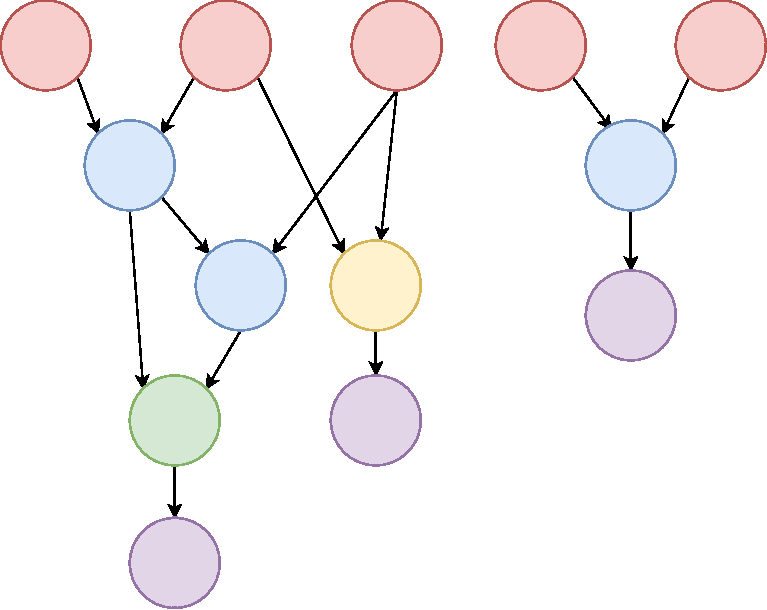
\includegraphics[width=75mm]{test.pdf}
  \caption{Sample test case}
  \label{fig:connect}
\end{figure}

The color coding is as follows:
\begin{itemize}
    \item Red : read nodes
    \item Blue : adder nodes
    \item Yellow : multiplier nodes
    \item Green : subtractor nodes
    \item Purple : write nodes
\end{itemize}

We have resource constraints and delays (in cycles) specified as:

\begin{center}
\begin{tabular}{ |c|c|c| } 
 \hline
 Operation type & Quantity & Delay \\ 
 \hline \hline
 Read & 2 & 3 \\ 
 \hline
 Adder & 2 & 2 \\ 
 \hline
 Subtractor & 1 & 1\\
 \hline
 Multiplier & 1 & 5\\
 \hline
 Write & 1 & 2\\
 \hline
\end{tabular}
\end{center}

Both graph and constraints format are shown in \ref{g}, and \ref{c} respectively. Output of the program can be seen in \ref{o}. We have specified dummy node using a type named 'C' and this 'C' type nodes can be used as cleanup and/or simplification gadgets for the scheduling problem. Let us first see the results then justify that it is the best that is possible given the input graph and the constraints on the graph. A visual representation of the output, corresponding to the specified color scheme, is shown in \ref{fig:sched};

\begin{figure}[!h]
  \centering
  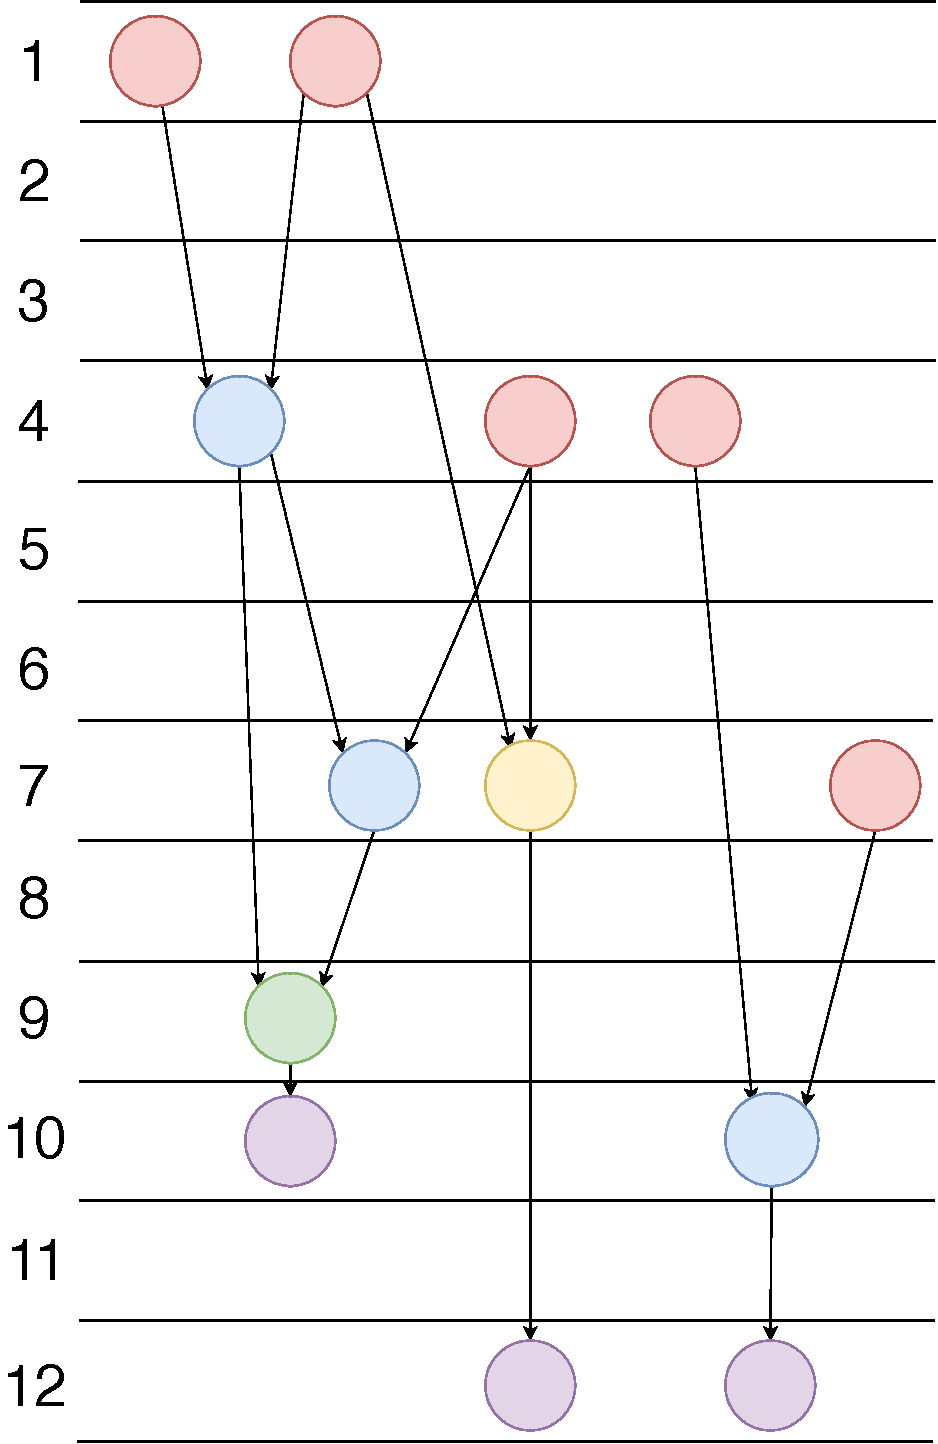
\includegraphics[width=80mm]{schedule.pdf}
  \caption{Result of the sample test case}
  \label{fig:sched}
\end{figure}

In this graph the nodes are shown based on only the schedule cycle and not the contiguous block of cycles where they would be executed. We observe that the program gave a resource constrained schedule using 12 cycles. Another observation is that the program was successfully able to independently provide schedules for the disconnected components. \\
It is easy to verify that no more than 2 read, 1 add, 1 subtract, 1 multiply and 1 write node is present in each cycle (considering the chunk of cycle where a node would be active). This covers the quantity constraint. Now, we also see that in any parent-child dependency where this dependency is captured by a forward arrow from parent to child, this child is only scheduled after all it's parents have completed, i.e. for every child the schedule obeys the rule that it is $>=$ parent schedule + parent's delay. This can be verified by observing that for every read node, it's child is scheduled only at 3rd or higher cycle relative to it's cycle. Similarly for add, subtract, multiple nodes. Thus we have justified that this is a valid schedule.\\
Now we need to prove that our algorithm gives a near-optimal result. Even for this sophisticated input graph, we show that the result i.e. 12 cycles is the minimum possible. There are many paths in this graph from red nodes to purple nodes. The one that is currently with minimum cycles is the one with read nodes in cycle 1, adder in cycle 4, adder in cycle 7, subtractor in cycle 9 and write node in cycle 10. This path/sequence is completed in 10 cycles. Other 2 write operations are place at cycle 12. If we try to reduce the scheduled cycles of other two write nodes, then the multiplier inputs must be scheduled in cycle 1. This contradicts the constraint that atmost 2 read operations can be performed in a cycle. Hence any schedule with < 12 cycles is not possible. 

\section{CONCLUSIONS}

In this work, we presented a resource-constrained scheduling algorithm, discussed the implementation level details and justified the correctness and optimiality of the program.

% \addtolength{\textheight}{-12cm}

%%%%%%%%%%%%%%%%%%%%%%%%%%%%%%%%%%%%%%%%%%%%%%%%%%%%%%%%%%%%%%%%%%%%%%%%%%%%%%%%
\onecolumn
\section{APPENDIX}

\subsection{Boost Graph definition used}
\label{typedef}
\begin{minted}{c}
typedef labeled_graph<adjacency_list<listS, vecS, bidirectionalS, Node>, string> Graph;
\end{minted}


\subsection{Ready list generator}
\label{ready}
\begin{minted}{c++}
vector<string> readyList(Graph& gr, char type){
    list<string> list;

    AdjGraph& underlying = gr.graph();
    typedef property_map<Graph, vertex_index_t>::type IndexMap;
    IndexMap index = get(vertex_index, underlying);

    pair<vertex_iter, vertex_iter> vp;
    for (vp = vertices(underlying); vp.first != vp.second; ++vp.first) {
        bool scheduled = schedule.find(V.at((int)index[*vp.first])) != schedule.end();
        if(scheduled)
            continue;
        if((int)in_degree(*vp.first, underlying) == 0 
            && V.at((int)index[*vp.first]).at(0) == type){
            list.push_back(V.at((int)index[*vp.first]));
        }
    }

    list.sort(mobilityComparator());
    vector<string> v{list.begin(), list.end()};
    return v;
}
\end{minted}

\subsection{Helper function for list scheduling}
\label{listhelp}
\begin{minted}{c++}
vector<string> listScheduleHelper(Graph& gcopy, char a){
    vector<string> ready = readyList(gcopy, a);
    vector<string> selected;

    int num_critical = 0;
    for(int i = 0; i < ready.size(); i++){
        if(mobility.at(ready.at(i)) == 0)
            num_critical++;
    }

    for(int i = 0; i < min(quantity.at(a), (int)ready.size()); i++){
        cout << ready.at(i) << endl;
        resource_num.insert(pair<string,int>(ready.at(i), i+1));
        selected.push_back(ready.at(i));
        int cycle = (inDegZero(ready.at(i))) ? last_cycle : 1;
        cout << "Start cycle : " << cycle << endl;
        // Determine last cycle of parents
        for(int j = 0; j < E_original.size(); j++){
            auto p = E_original.at(j);
            if(p.second == ready.at(i) && schedule.find(p.first) != schedule.end())
                cycle = max(cycle, schedule.at(p.first) + delay.at(p.first.at(0)));
        }
        schedule.insert(pair<string,int>(ready.at(i), cycle));
        last_cycle = max(last_cycle, cycle);
        cout << "Given schedule " << cycle << " to " << ready.at(i) << endl;
    }

    return selected;
}
\end{minted}

\subsection{Overall code for List scheduling}
\label{list}
\begin{minted}{c++}
void listSchedule(){
    int cycle = 1;
    vector<string> remove;
    int limit = 1;
    bool done;

    while(limit != 0 || !done){
        Graph g;
        parseGraph(g, "graph2.txt");
        printGraph();
        ASAP(g);
        printASAP();
        ALAP(g);
        printALAP();
        computeMobilities();
        printMobilities();
        remove.clear();
        for(char a : {'C', 'A', 'S', 'M', 'R', 'W'}){
            vector<string> r = listScheduleHelper(g, a);
            remove.insert(std::end(remove), std::begin(r), std::end(r));
        }
        done = removeVertices(g, remove);
        if(done){
            schedule.insert(pair<string, int>(V.at(0), 0));
            resource_num.insert(pair<string,int>(V.at(0), 1));
            break;
        }
        writeGraph("graph2.txt");
        limit = num_vertices(g);
    }    
}
\end{minted}

\subsection{Test Graph}
\label{g}
R 3 A 1 \\
R 4 A 1\\
A 1 A 2\\
R 5 A 2\\
A 1 S 1\\
A 2 S 1\\
R 6 A 3\\
R 7 A 3\\
S 1 W 1\\
A 3 W 2\\
R 5 M 1\\
R 4 M 1\\
M 1 W 3\\

\subsection{Test Constraints}
\label{c}%
C 10 1\\
A 2 2\\
S 1 1\\
M 1 5\\
R 2 3\\
W 1 2\\

\subsection{Output for test case}
\label{o}%
Node    Cycle   Resource number\\
R3      1       1\\
A1      4       1\\
R4      1       2\\
A2      7       1\\
R5      4       1\\
S1      9       1\\
R6      4       2\\
A3      10      1\\
R7      7       1\\
W1      10      1\\
W2      12      1\\
M1      7       1\\
W3      12      1\\


%%%%%%%%%%%%%%%%%%%%%%%%%%%%%%%%%%%%%%%%%%%%%%%%%%%%%%%%%%%%%%%%%%%%%%%%%%%%%%%%


\end{document}
